\documentclass{beamer}

\usepackage[frenchb]{babel}
\usepackage[T1]{fontenc}
\usepackage[latin1]{inputenc}
\usetheme{AnnArbor}
\usepackage{graphicx}

\title{Soutenance du projet de programmation : La Ruche}
\date{31 Mai 2017}
\author[1]{Brigon Enzo \and Davtyan Narek \and Douard Amelina \and Grand Maxence \and Hadjadj Lies \and Muller Lucie }


\begin{document}

\begin{frame}
  \titlepage
\end{frame}

\begin{frame}
  \tableofcontents[]
\end{frame}

\section{Introduction}%1 minutes
%rappel des rêgles

\begin{frame}
\begin{itemize}
\frametitle{Rappel des r\`egles}
\item Jeu \`a deux joueurs
\item Entourer la reine adverse
\item Chaque pi\`eces poss\`edent ses propres coups
\item Respect de l'unicit\'e de la ruche
\end{itemize}
\end{frame}

\section{Repr\'esentation des donn\'ees}
  \begin{frame}
      %\frametitle{Repr\'esentation des Insectes}
  \end{frame}
    \begin{frame}
        %\frametitle{Repr\'esentation des Insectes}
        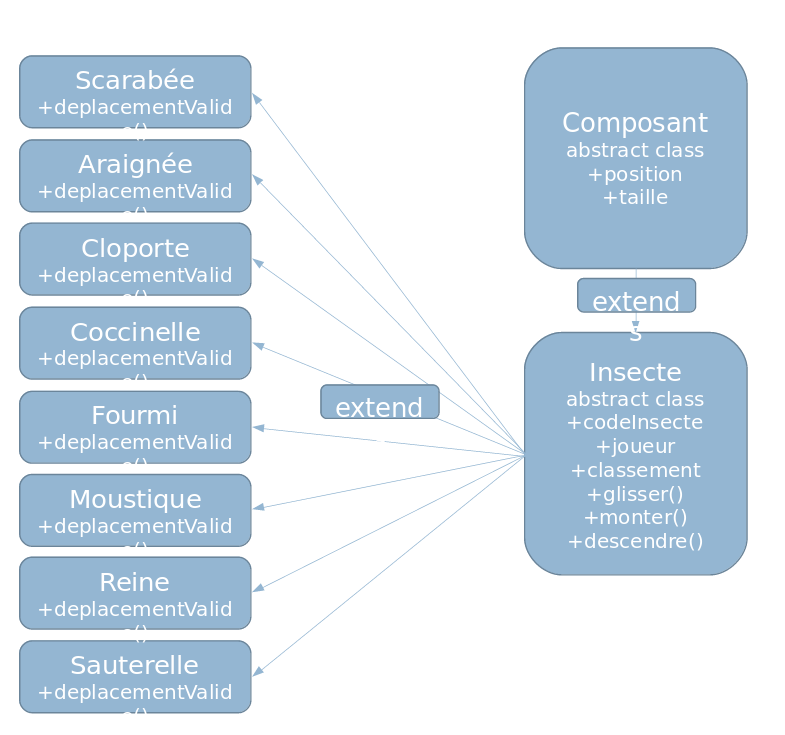
\includegraphics[width=10cm]{insecteRepres.png}
    \end{frame}
    \begin{frame}
        \frametitle{Repr\'esentation du Plateau}
        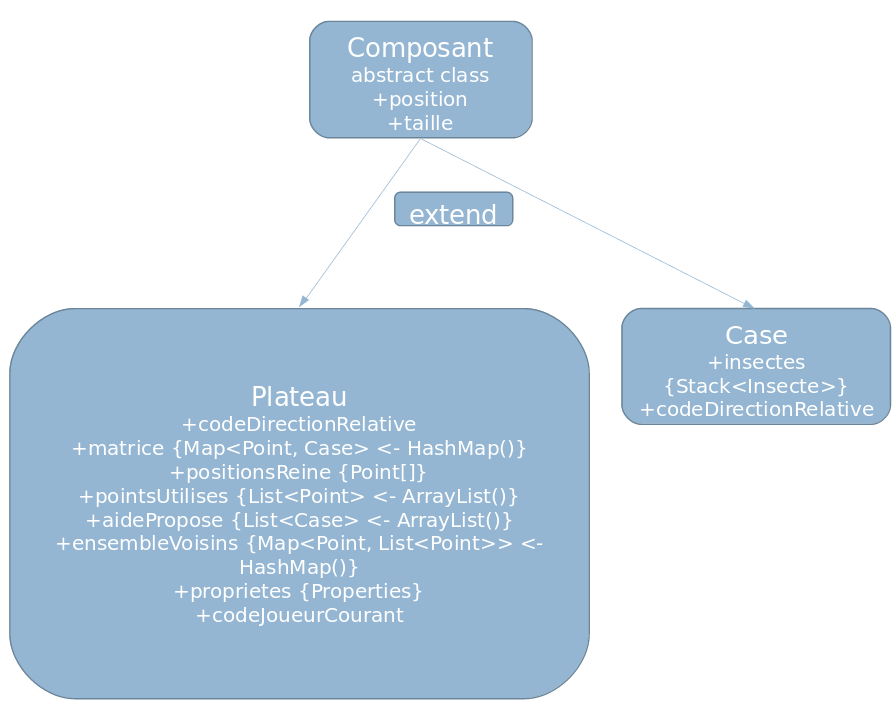
\includegraphics[width=10cm]{plaeayRepres.png}
    \end{frame}
    \begin{frame}
        \frametitle{Repr\'esentation du Plateau}
        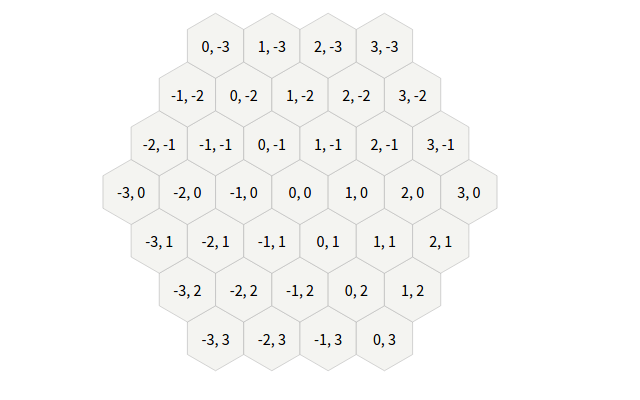
\includegraphics[width=10cm]{./grid.png}
    \end{frame}
    \begin{frame}
        \frametitle{Repr\'esentation des Coups}
        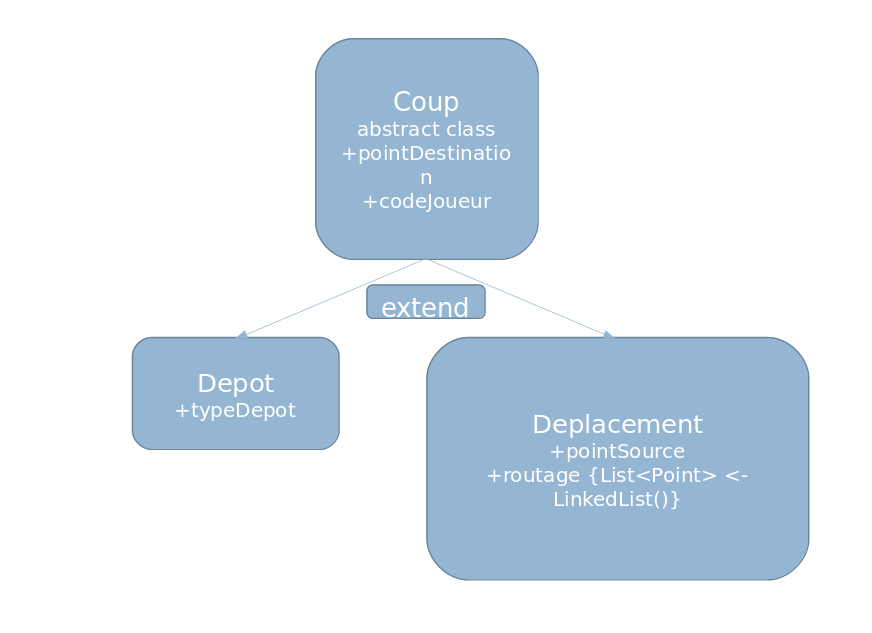
\includegraphics[width=10cm]{./coupRepres.png}
    \end{frame}
    \begin{frame}
        \frametitle{Probl\`eme d'unicit\'e}
    \end{frame}
    \begin{frame}
        \frametitle{Probl\`eme d'unicit\'e}
        \begin{center}
        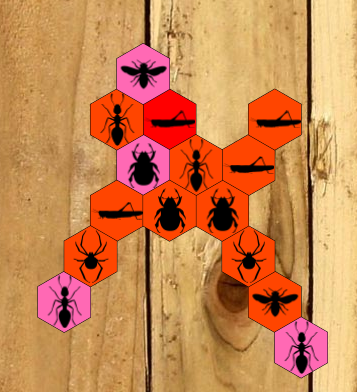
\includegraphics[width=6cm]{./graphe.png}
        \end{center}
    \end{frame}
    \begin{frame}
        \frametitle{Probl\`eme d'unicit\'e}
        \begin{center}
        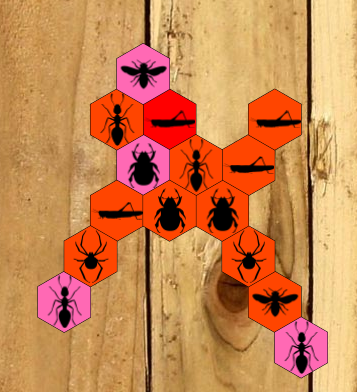
\includegraphics[width=6cm]{./graphe.png}
        \end{center}
    \end{frame}
    \begin{frame}
        \frametitle{Probl\`eme d'unicit\'e}
        \begin{center}
        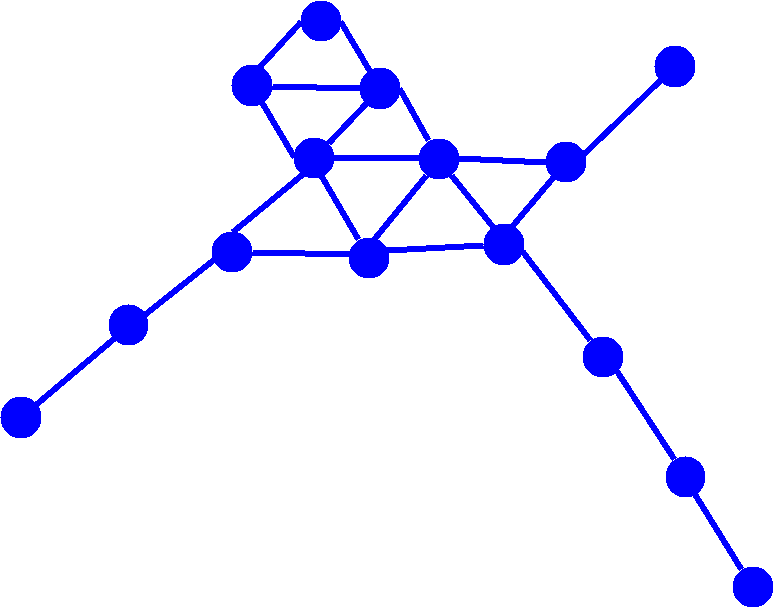
\includegraphics[width=7cm]{./graphe2.png}
        \end{center}
    \end{frame}
    \begin{frame}
        \frametitle{Probl\`eme d'unicit\'e}
        \begin{itemize}
        \item Equation de r\'ecurrence : \[ V_{ij}^t = (V_{ix}^{t+1} . V_{xj}^{t+1}) + V_{ij}^{t+1}  \]
        \end{itemize}
    \end{frame}
    \begin{frame}
        \frametitle{Probl\`eme d'unicit\'e}
        \begin{itemize}
        \item Equation de r\'ecurrence : \[ V_{ij}^t = (V_{ix}^{t+1} . V_{xj}^{t+1}) + V_{ij}^{t+1}  \]
        \item Union Find
        \end{itemize}
    \end{frame}
    \begin{frame}
        \frametitle{Probl\`eme d'unicit\'e}
        \begin{center}
        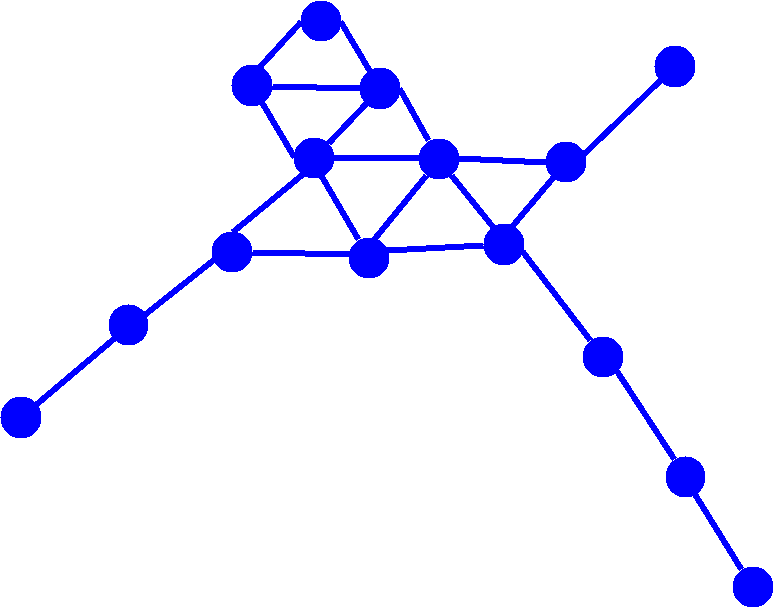
\includegraphics[width=7cm]{./graphe2.png}
        \end{center}
    \end{frame}
    \begin{frame}
        \frametitle{Probl\`eme d'unicit\'e}
        \begin{center}
        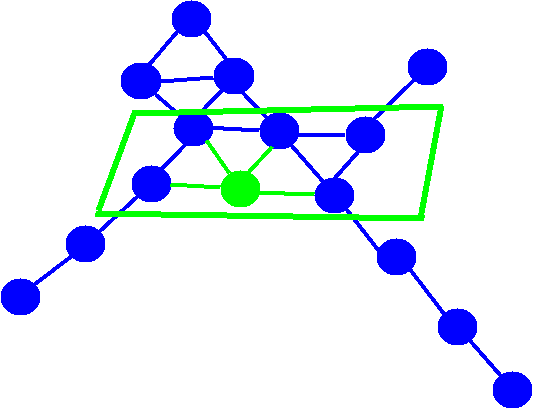
\includegraphics[width=7cm]{./voisinsConnexe.png}
        \end{center}
    \end{frame}
    \begin{frame}
        \frametitle{Probl\`eme d'unicit\'e}
        \begin{center}
        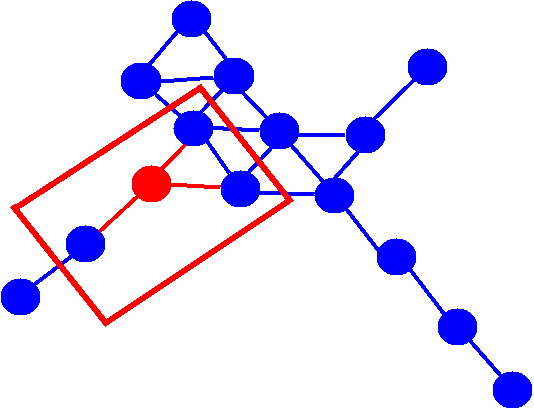
\includegraphics[width=7cm]{./voisinNonConnexe.png}
        \end{center}
    \end{frame}
    \begin{frame}
        \frametitle{Probl\`eme d'unicit\'e}
        \begin{center}
        \includegraphics[width=4cm]{./2voisins.png}
        \includegraphics[width=2cm]{./3voisins.png}
        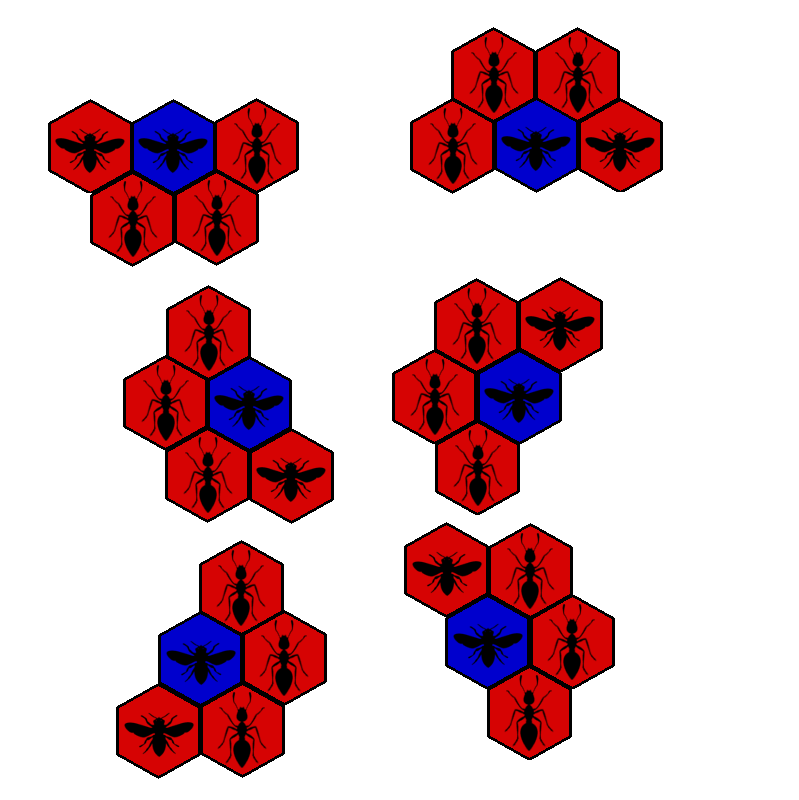
\includegraphics[width=3cm]{./4voisins.png}
        \end{center}
    \end{frame}



\section{Interraction Homme Machine \& Fonctionnalit\'ees}%16 min
\begin{frame}
\end{frame}\begin{frame}
    \frametitle{Pr\'esentation g\'en\'erale de l'IHM}
\end{frame}
    \begin{frame}
        \frametitle{Pr\'esentation g\'en\'erale de l'IHM}
        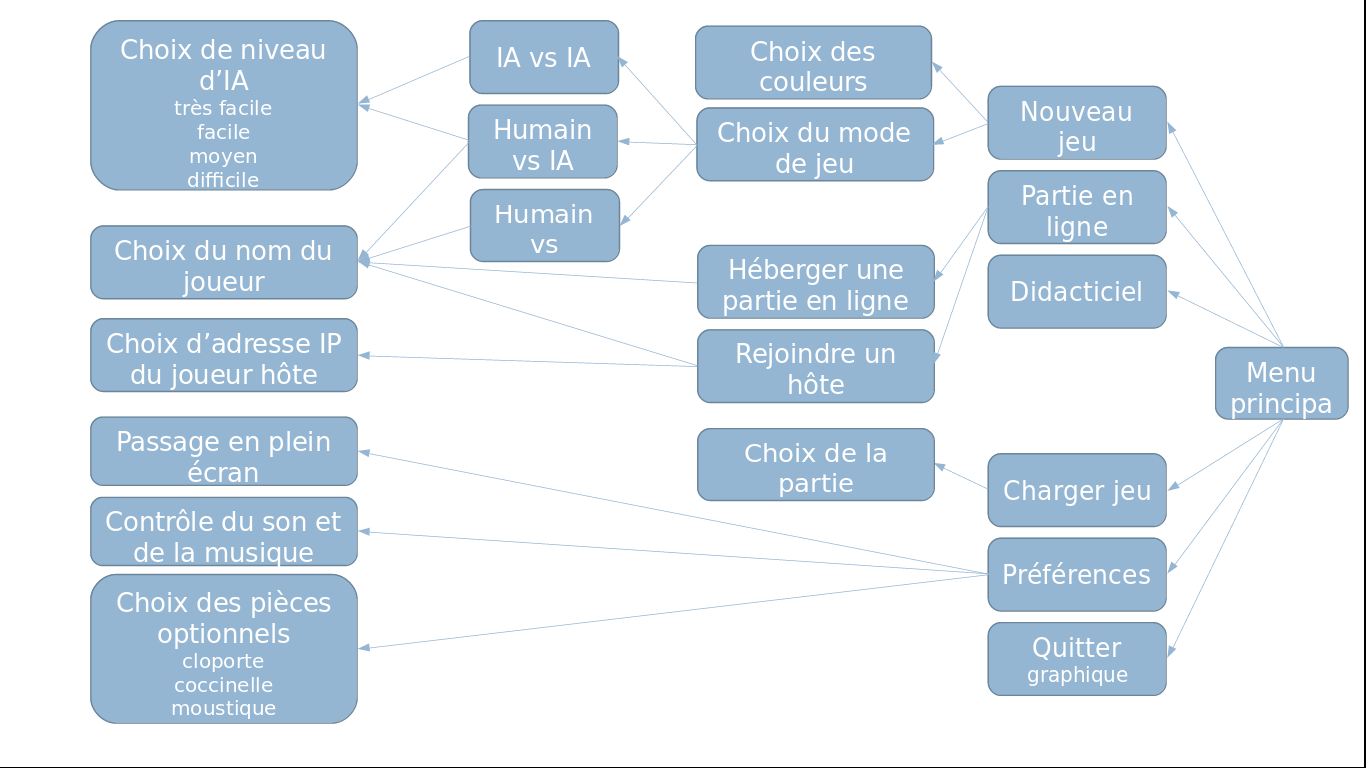
\includegraphics[width=10cm]{general.png}
    \end{frame}
    \begin{frame}
        \frametitle{Partie en local}
        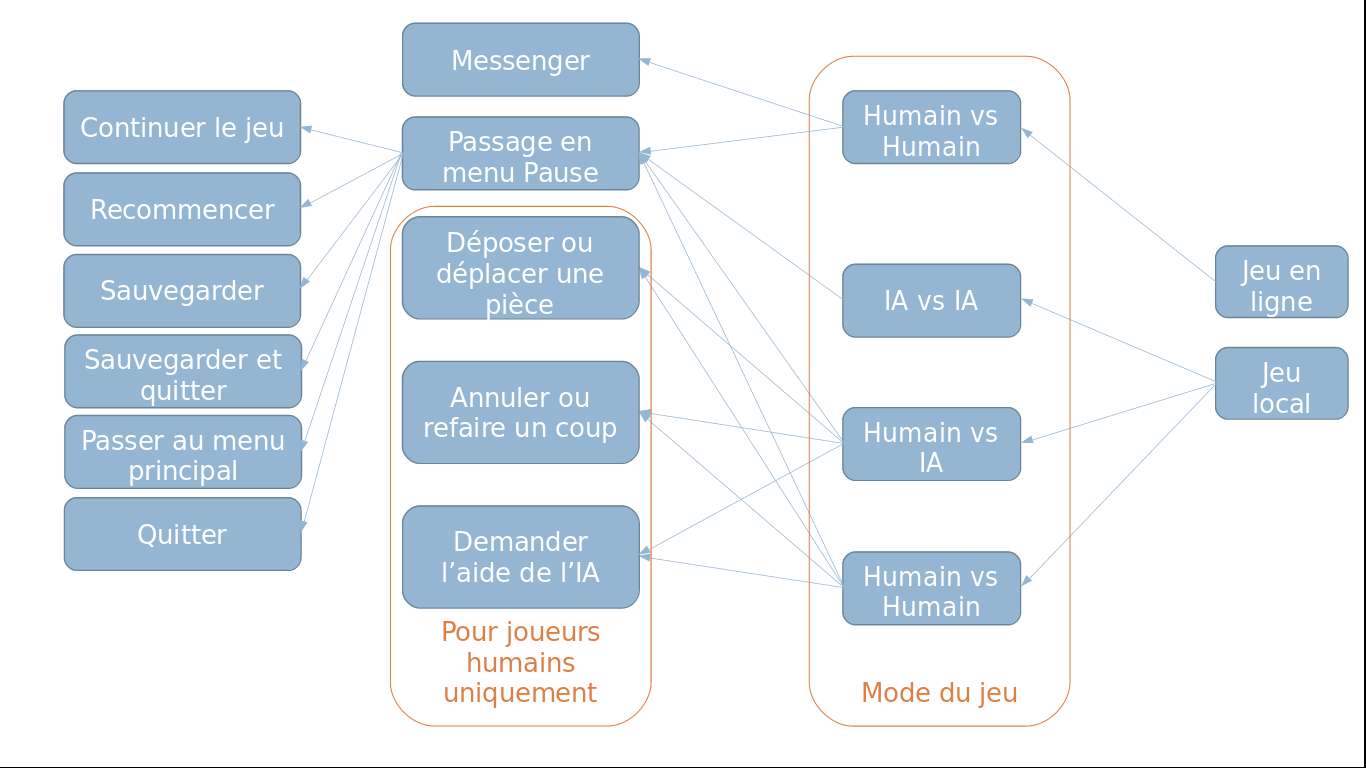
\includegraphics[width=10cm]{deroulementPartie.png}
    \end{frame}
    \begin{frame}
      \frametitle{Sauvegarde \& Chargment}
    \end{frame}
    \begin{frame}
      \frametitle{Sauvegarde \& Chargment}
      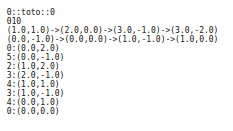
\includegraphics[width=7cm]{./charge.png}
    \end{frame}
    \begin{frame}
      \frametitle{Sauvegarde \& Chargment}
      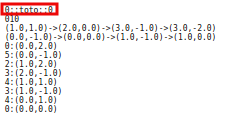
\includegraphics[width=7cm]{./chargeGen.png}
    \end{frame}
    \begin{frame}
      \frametitle{Sauvegarde \& Chargment}
      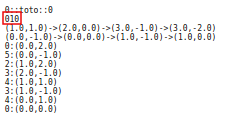
\includegraphics[width=7cm]{./chargeIns.png}
    \end{frame}
    \begin{frame}
      \frametitle{Sauvegarde \& Chargment}
      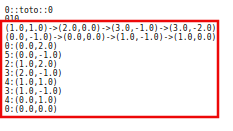
\includegraphics[width=7cm]{./chargeCoup.png}
    \end{frame}
    \begin{frame}
        \frametitle{Partie en r\'eseau}
    \end{frame}
    \begin{frame}
        \frametitle{Partie en r\'eseau}
        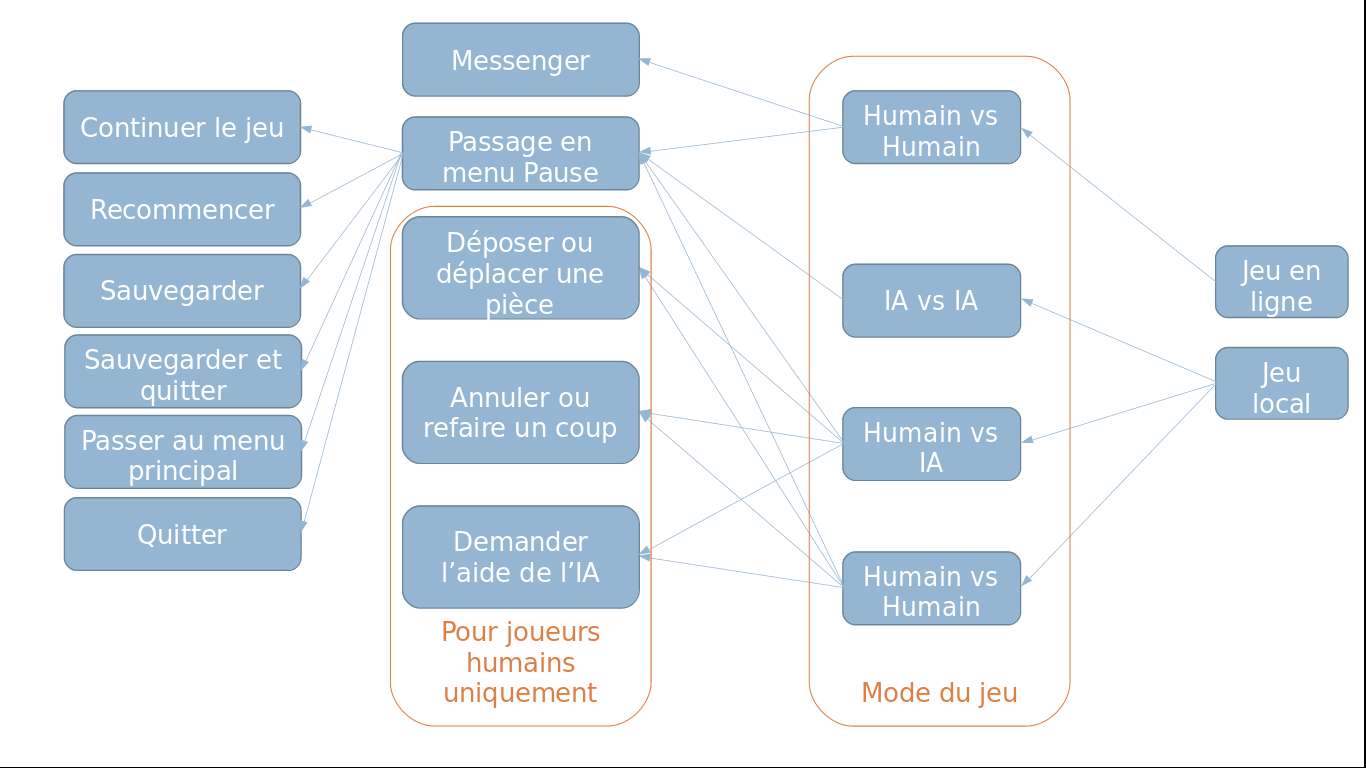
\includegraphics[width=10cm]{deroulementPartie.png}
    \end{frame}
    \begin{frame}
        \frametitle{Partie en r\'eseau}
        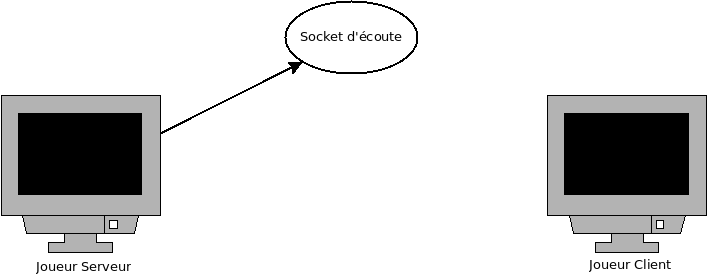
\includegraphics[width=10cm]{ecoute.png}
    \end{frame}
    \begin{frame}
        \frametitle{Partie en r\'eseau}
        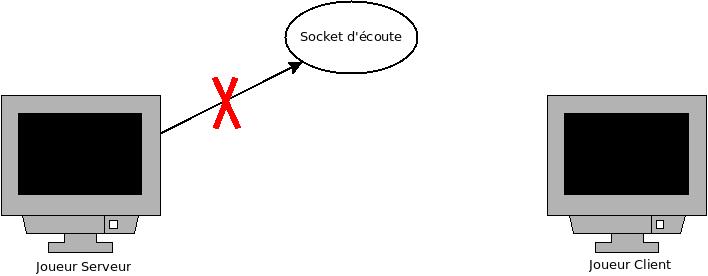
\includegraphics[width=10cm]{annuation.png}
    \end{frame}
    \begin{frame}
        \frametitle{Partie en r\'eseau}
        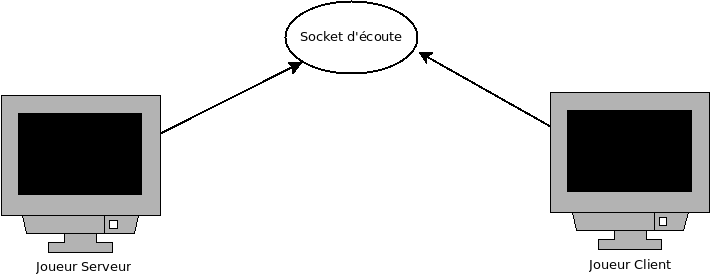
\includegraphics[width=10cm]{accept.png}
    \end{frame}
    \begin{frame}
        \frametitle{Partie en r\'eseau}
        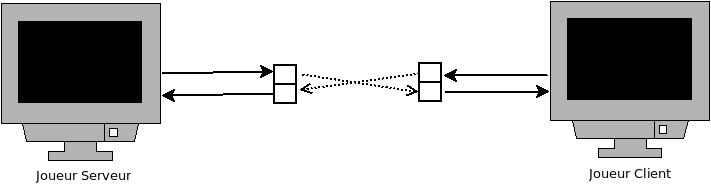
\includegraphics[width=10cm]{echange.png}
    \end{frame}
    \begin{frame}
        \frametitle{Partie en r\'eseau}
        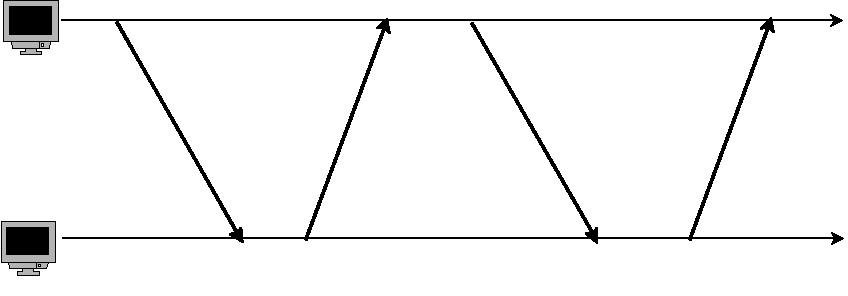
\includegraphics[width=10cm]{echangeOK.png}
    \end{frame}
    \begin{frame}
        \frametitle{Partie en r\'eseau}
        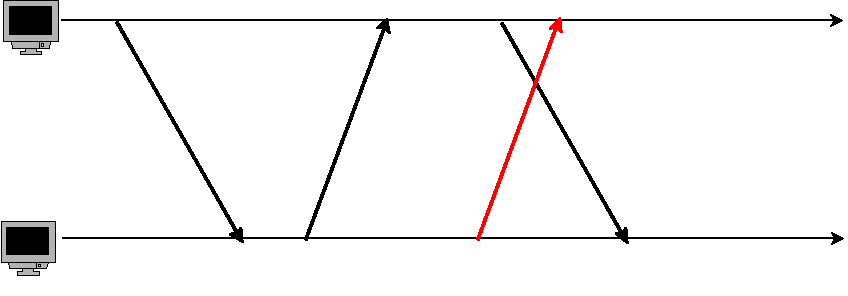
\includegraphics[width=10cm]{echangeBUG.png}
    \end{frame}




\section{\'Evolution de l'IHM et Tests utilisateurs}%2 min
\begin{frame}
\end{frame}
\begin{frame}
    \frametitle{Menu Principale}
\end{frame}
\begin{frame}
    \frametitle{Menu Principale}
    \begin{center}
    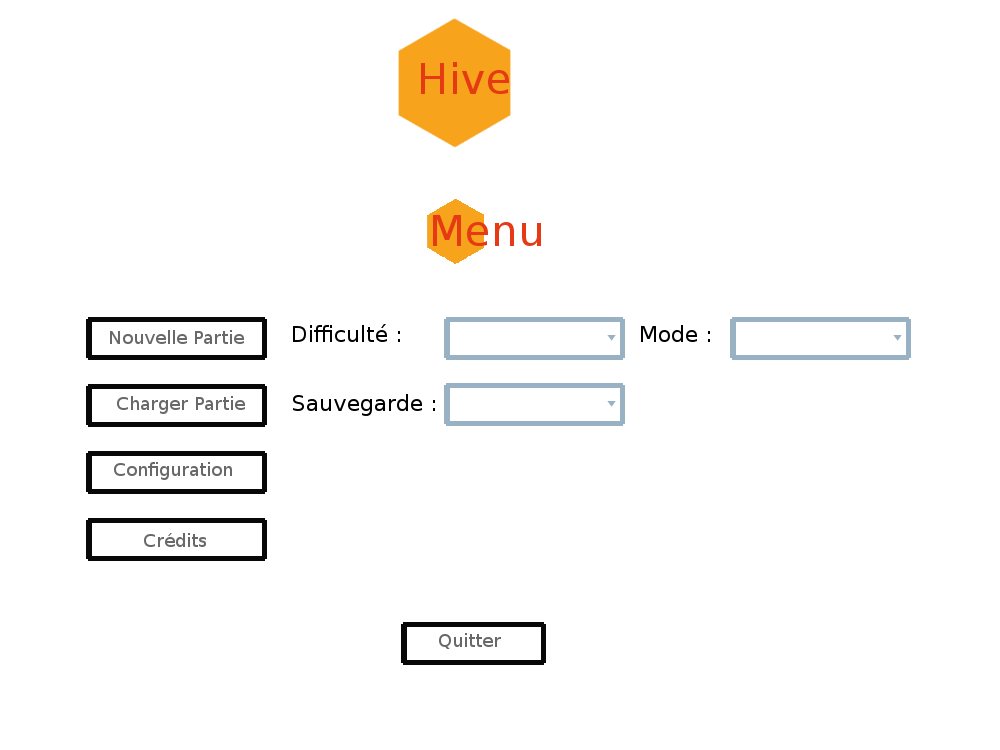
\includegraphics[width=7cm]{menuPrincipalv1.png}
    \end{center}
\end{frame}

\begin{frame}
    \frametitle{Menu Principale}
    \begin{center}
    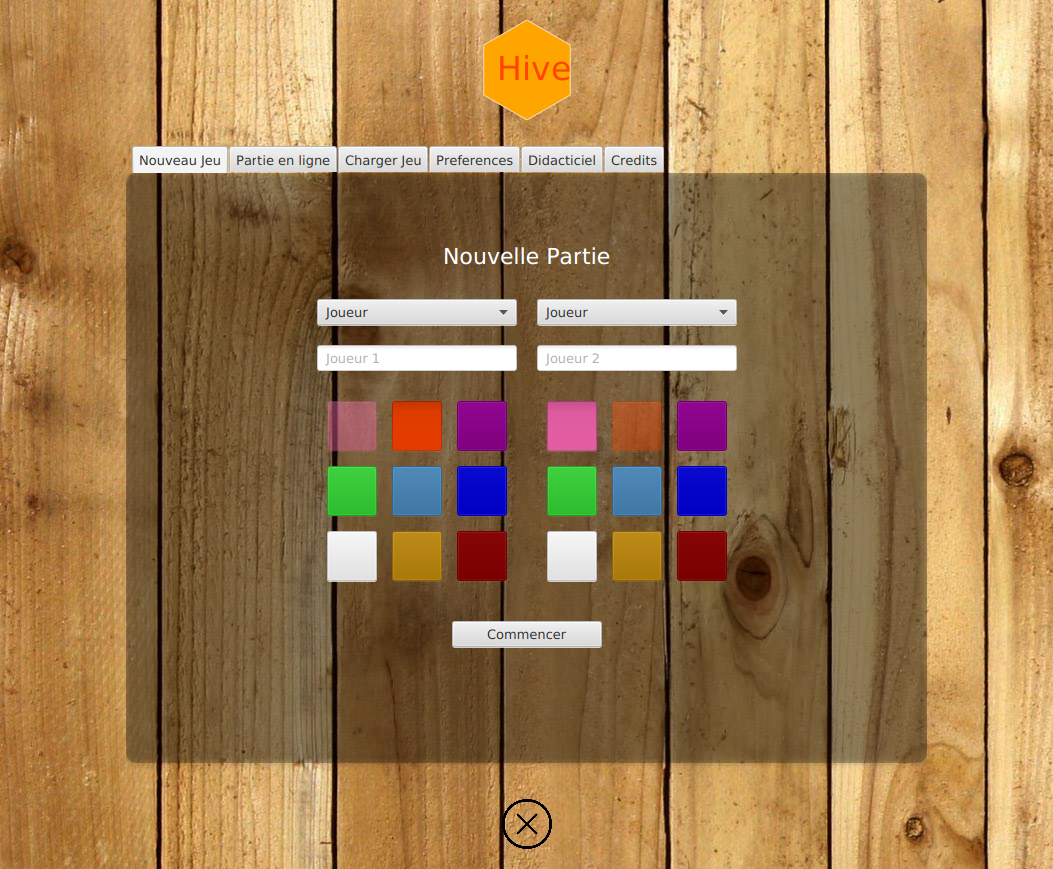
\includegraphics[width=7cm]{menu.png}
    \end{center}
\end{frame}
\begin{frame}
    \frametitle{Menu Principale}
    \begin{center}
    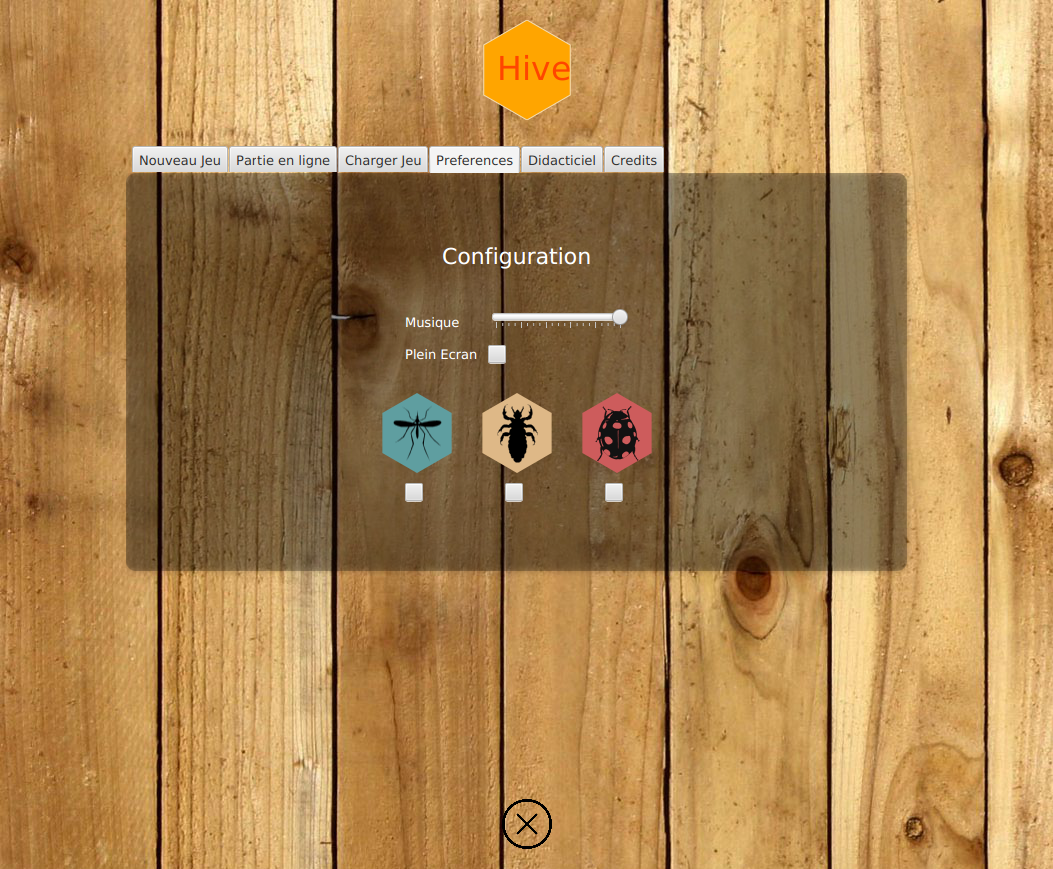
\includegraphics[width=7cm]{preferences.png}
    \end{center}
\end{frame}
\begin{frame}
    \frametitle{Menu Principale}
    \begin{center}
    \includegraphics[width=7cm]{PartieEnLigne.png}
    \end{center}
\end{frame}
\begin{frame}
    \frametitle{L'interface du jeu}
\end{frame}
\begin{frame}
    \frametitle{L'interface du jeu}
    \begin{center}
    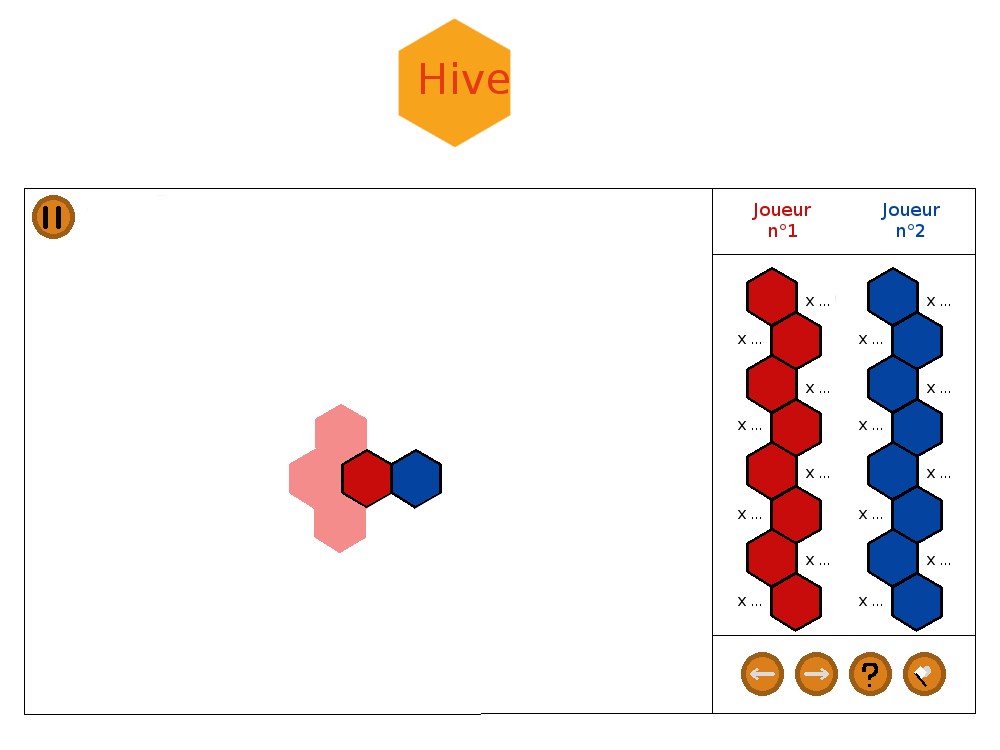
\includegraphics[width=7cm]{jeuv1.png}
    \end{center}
\end{frame}
\begin{frame}
    \frametitle{L'interface du jeu}
    \begin{center}
    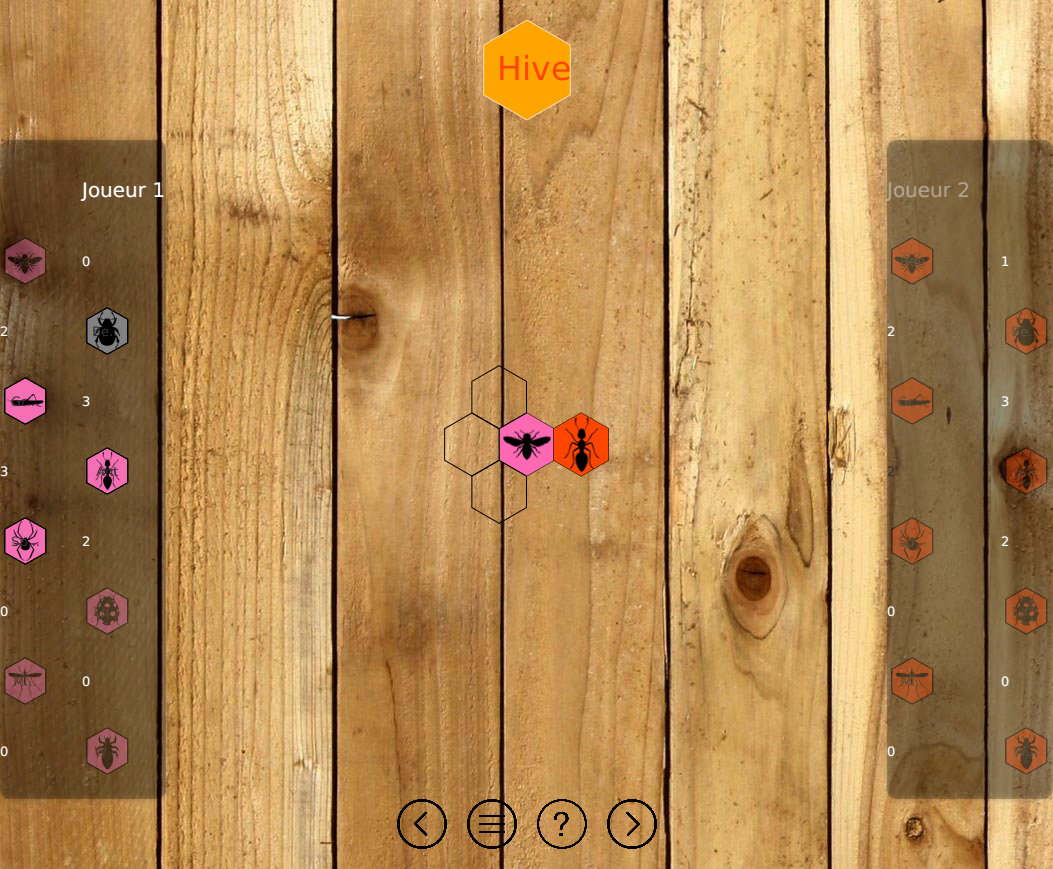
\includegraphics[width=7cm]{jeu.png}
    \end{center}
\end{frame}
\begin{frame}
    \frametitle{L'interface du jeu}
    \begin{center}
    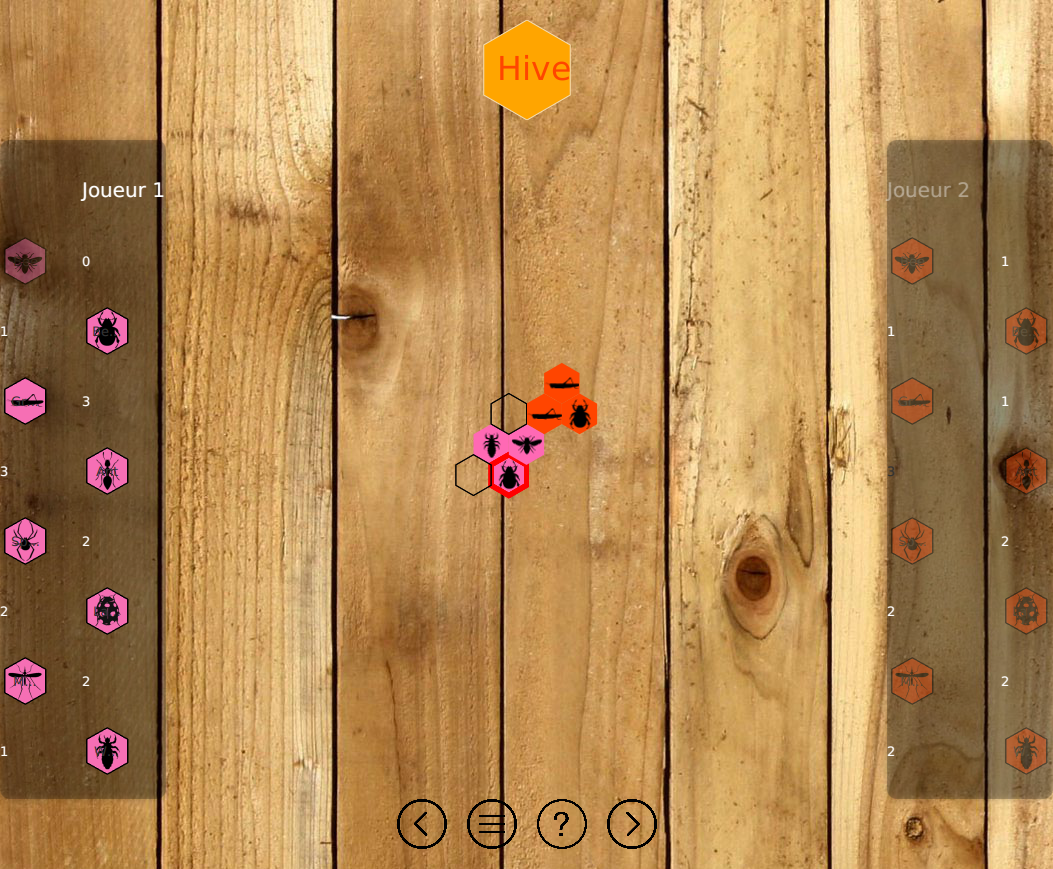
\includegraphics[width=7cm]{deplCloporte.png}
    \end{center}
\end{frame}


\section{Intelligence Artificielle}%8minutes

\begin{frame}
\frametitle{Les diff\'erents niveaux de difficult\'e}
\begin{itemize}
\item Tr\`es Facile
\item Facile
\item Moyen
\item Difficile
\end{itemize}
\end{frame}


\begin{frame}
\frametitle{V\'erification du niveau des IA}
\begin{center}
\includegraphics[width=7cm]{./TresFacFac.png}
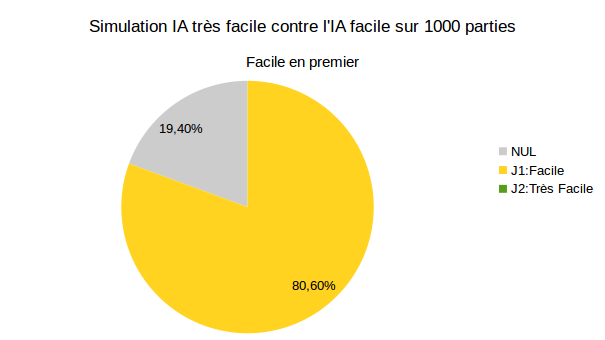
\includegraphics[width=7cm]{./FacTresFac.png}
\end{center}
\end{frame}

\begin{frame}
\frametitle{V\'erification du niveau des IA}
\begin{center}
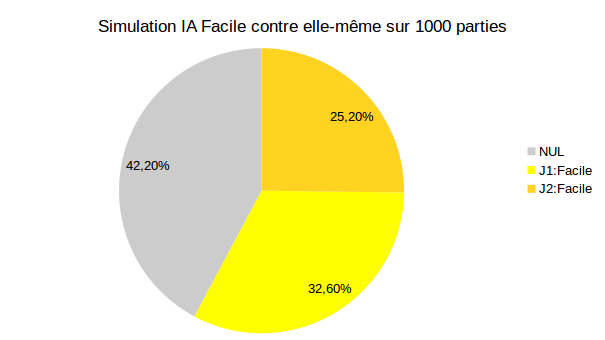
\includegraphics[width=7cm]{./MoyFac.png}
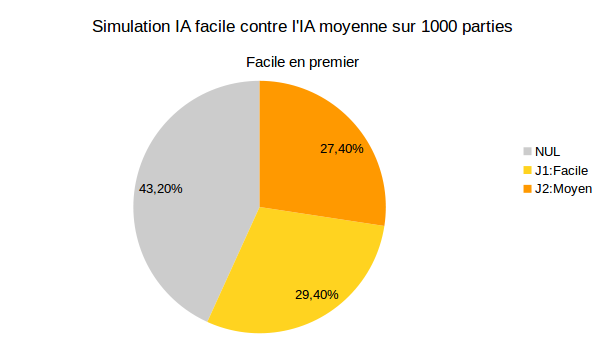
\includegraphics[width=7cm]{./FacMoy.png}
\end{center}
\end{frame}

\begin{frame}
\frametitle{V\'erification du niveau des IA}
\begin{center}
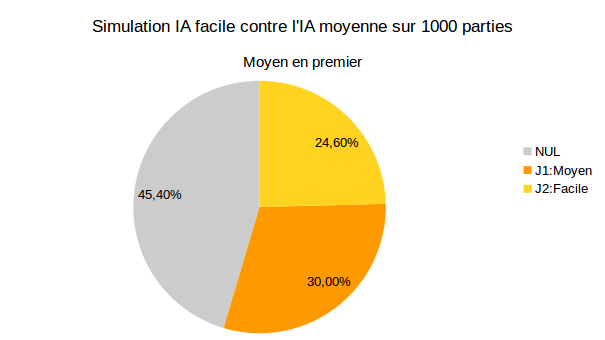
\includegraphics[width=7cm]{./TresFacTresFac.png}
\end{center}
\end{frame}
\section{Quelques pistes d'am\'elioration}%1 minute

\begin{frame}
\frametitle{Pour l'IHM}
\end{frame}
\begin{frame}
\frametitle{Pour les fonctionnalit\'ees}
\begin{itemize}
\item Jeu \`a deux joueurs
\item Partie en r\'eseau sur un serveur externe
\item Syst\`eme de profils
\end{itemize}
\end{frame}

\begin{frame}
\frametitle{Pour l'IA}
\end{frame}

\end{document}
